% !TEX program = xelatex
% ============================================================
%  TROMLEORKESTRET — Booking Sheet
%  Compile with:  xelatex main.tex   (run twice)
%
%  This file is meant to be edited by hand. The sections you'll
%  most likely want to change are marked  %%% EDIT ME
%
%  Overleaf: the "% !TEX program = xelatex" line above should make
%  Overleaf pick XeLaTeX automatically. If it still tries pdfLaTeX,
%  set it manually: Menu (top left) -> Settings -> Compiler -> XeLaTeX.
% ============================================================
\documentclass[10pt]{article}

% ---------- Page geometry ----------
\usepackage{geometry}
\geometry{a4paper, margin=14mm, top=0mm, bottom=9mm}

% ---------- Fonts (xelatex, system fonts) ----------
\usepackage{fontspec}
\setmainfont{Lora}[Mapping=tex-text]
\IfFontExistsTF{Bitstream Charter}
  {\newfontfamily\serifreader{Bitstream Charter}[Mapping=tex-text]}
  {\newfontfamily\serifreader{Charter}[Mapping=tex-text]} % macOS name
\newfontfamily\labelfont{DejaVu Sans Condensed}[Mapping=tex-text]

% ---------- Colour palette ----------
\usepackage[table]{xcolor}
\definecolor{bg}{HTML}{14110D}       % page background
\definecolor{cream}{HTML}{EBE2D0}    % body text
\definecolor{brightcream}{HTML}{F3E9D2} % headings / titles
\definecolor{brass}{HTML}{C59D5F}    % accent gold
\definecolor{ember}{HTML}{C1440E}    % accent rust/orange
\definecolor{muted}{HTML}{9C8A66}    % dim labels
\definecolor{bodytext}{HTML}{D8CBAF} % paragraph grey-cream
\definecolor{hairline}{HTML}{6E5F45} % faint rules

% ---------- Full-bleed dark background ----------
% NOTE: this is painted explicitly at the top of each page (see \bgfill
% below) rather than via eso-pic's per-page shipout hook, which does not
% repaint reliably on every page in combination with hyperref.
\newcommand{\bgfill}{%
  \begin{tikzpicture}[remember picture, overlay]
    \fill[bg] (current page.south west) rectangle (current page.north east);
  \end{tikzpicture}%
}

% ---------- Images / drawing ----------
\usepackage{graphicx}
\usepackage{tikz}
\usetikzlibrary{calc}

% ---------- Tables / lists ----------
\usepackage{array}
\usepackage{tabularx}
\usepackage{enumitem}
\usepackage{tcolorbox}
\tcbuselibrary{skins}

% ---------- Links ----------
\usepackage{hyperref}
\hypersetup{%
  colorlinks=true, urlcolor=brass, linkcolor=brass,
  pdfborder={0 0 0}, pdfborderstyle={/S/U /W 0}, hidelinks=false,
  breaklinks=true,
  pdftitle={Tromleorkestret -- Booking Sheet}%
}
% belt-and-braces: some PDF viewers still draw a hover/focus rectangle around
% link annotations even with pdfborder 0 0 0 --- this removes the annotation
% border style entirely so links read as plain coloured text, not a button.
\hypersetup{linkbordercolor=bg, citebordercolor=bg, filebordercolor=bg, urlbordercolor=bg}

% Link style matching the CV (cv_7.tex / moderncv "casual"): plain
% coloured hyperlink text, no icon --- \homepagesymbol etc. are actually
% empty in that style, so there was never an icon glyph, just \href{url}
% {\color{...}text}. Brass here instead of the CV's literal blue, to match
% this document's palette.
\newcommand{\cvlink}[2]{\href{#1}{\color{brass}#2}}

\setlength{\parindent}{0pt}
\setlength{\parskip}{0pt}
\pagestyle{empty}

% ---------- Small helpers ----------
% Section eyebrow heading, e.g. \eyebrow{The Machine}
\newcommand{\eyebrow}[1]{{\labelfont\fontsize{10}{12}\selectfont\color{ember}\MakeUppercase{#1}}}
% Muted small-caps label, e.g. rider table keys
\newcommand{\rlabel}[1]{{\labelfont\fontsize{7.6}{9}\selectfont\color{brass}\MakeUppercase{#1}}}

\begin{document}
\color{cream}

% ================================================================
%  PAGE 1
% ================================================================
\bgfill

% ---- Hero image + title, full page width, absolute positioning ----
\begin{tikzpicture}[remember picture, overlay]
  \node[anchor=north west, inner sep=0pt] at (current page.north west)
    {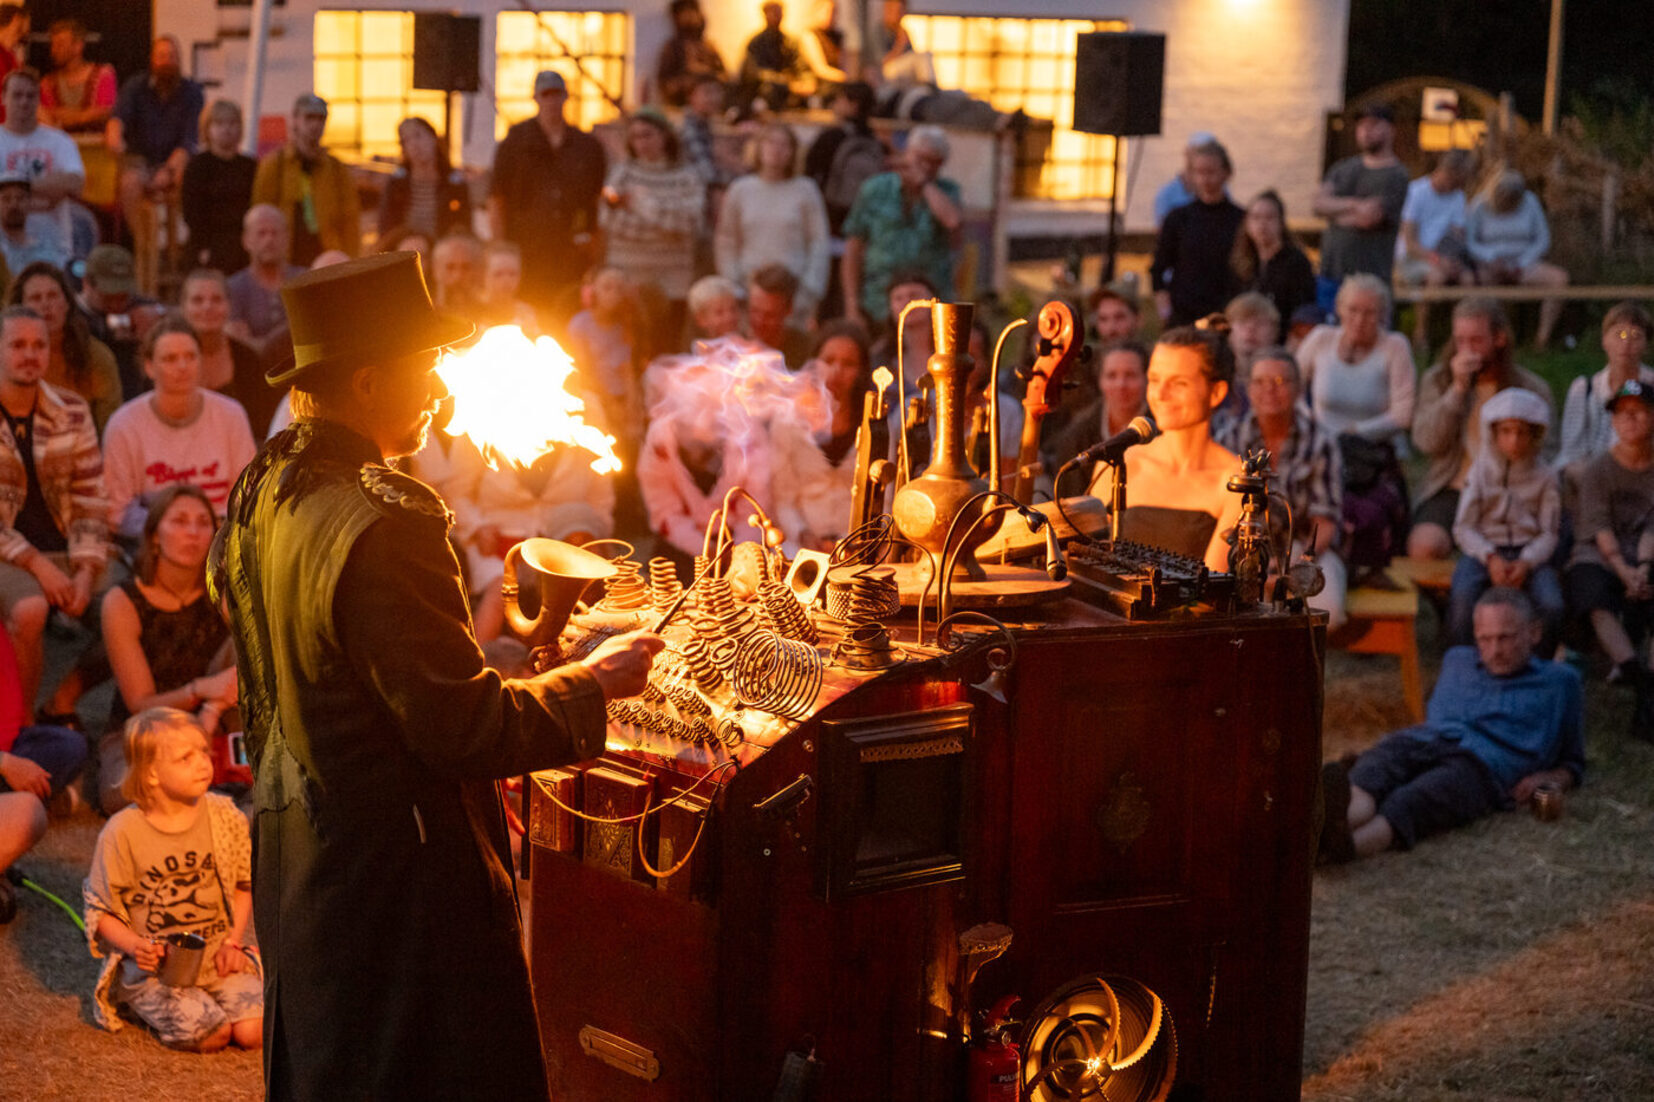
\includegraphics[width=\paperwidth]{img/hero_crop.jpg}};
  \node[anchor=north west, inner sep=0pt] at (current page.north west)
    {
\includegraphics[width=\paperwidth]{img/hero_gradient.png}};

  % thin brass frame, inset from the page edge
  \draw[brass, opacity=0.55, line width=0.5pt]
    ($(current page.north west)+(6mm,-6mm)$) rectangle
    ($(current page.north west)+(\paperwidth-6mm,-134mm)$);

  % kicker --- sits on a small dark pill so it stays legible over any photo
  \node[anchor=north west, inner sep=1.6mm, fill=bg, fill opacity=0.6,
        text opacity=1, rounded corners=1pt,
        xshift=12.5mm, yshift=-10.5mm] at (current page.north west)
    {\labelfont\fontsize{8.4}{10}\selectfont\bfseries\color{brightcream}
     {\color{ember}\textbullet}\ \ BOOKING SHEET};

  % title + subtitle
  \node[anchor=north west, inner sep=0pt] at
    ($(current page.north west)+(14mm,-106mm)$)
    {%
      \begin{minipage}[t]{160mm}
        {\fontsize{40}{40}\selectfont\itshape\bfseries\color{brightcream} Tromleorkestret}\\[4mm]
        {\labelfont\fontsize{15}{20}\selectfont\color{cream}
         The Fire-Breathing Music Machine
        }
      \end{minipage}%
    };
\end{tikzpicture}

\vspace*{140mm} % reserves the space the hero image occupies (image renders ~140mm tall at full page width)

% ---- location / founded / url band ----
\vspace{-8mm}
\noindent
{\labelfont\fontsize{11.5}{14}\selectfont\color{muted}%
  CHRISTIANIA, DENMARK \quad{\color{ember}\textbullet}\quad FOUNDED 2012 \quad{\color{ember}\textbullet}\quad TROMLEORKESTRET.COM}

\vspace{2mm}
\noindent
%%% EDIT ME — the opening description
{\serifreader\fontsize{12}{18}\selectfont\color{cream}
\textbf{Tromleorkestret} is two people and a homebuilt music machine. The 
Trio plays psychedelic barrel-organ music on self-constructed, 
mechanical, high-tech instruments. The performance is a celebration of  man's 
ability to create machines that  can perform actions that humans are not capable 
of, leading ideas to new heights. Just as well as it is a doomsday prophecy 
about the  machines' inevitable takeover of human consciousness.
\par}

\vspace{3mm}
{\color{hairline}\hrule height 0.4pt}
\vspace{3mm}

% ---- The Machine / The Performance ----      %%% EDIT ME
\noindent
\begin{minipage}[t]{0.485\linewidth}
  {\labelfont\fontsize{10.8}{13}\selectfont\color{ember}\MakeUppercase{The Machine}}\\[2mm]
  {\serifreader\fontsize{10.5}{15.2}\selectfont\color{bodytext}
   The machine is built by the two musicians. A never ending projekt that has beeing
   developing for 14 years so far. It has a robotic slide bass, mechanical xylophone,
   drums and keybord, a percussion instrument based on amplified springs and
   flamethrowers spewing fire in sync with the music. The sound is manipulated
   wirelessly by a pair of gloves, featuring real-time effects, ranging from reversers
   to granular spaces.
\par}
\end{minipage}%
\hfill
\begin{minipage}[t]{0.485\linewidth}
  {\labelfont\fontsize{10.8}{13}\selectfont\color{ember}\MakeUppercase{The Performance}}\\[2mm]
  {\serifreader\fontsize{10.5}{15.2}\selectfont\color{bodytext}
  The fusion of sound, light, pyrotechnics and movement creates a doorway into
  a psychedelic experience. The visual universe has references to steampunk while the
  music draws lines from krautrock, psychedelic jazz and experimental
  electronic music in an ever evolving soundscape. The interaction between
  improvisational musicians and the robotic instruments blurs the barriers
  between man and machine.
  \par}
\end{minipage}

\vspace{11mm}

% ---- detail photo with caption ----
% (img/detail_crop.jpg is pre-cropped to a 182x30mm banner --- see img/README.md
%  if you swap in a different source photo, re-crop it to the same ratio first)
\noindent
\begin{tikzpicture}
  \node[anchor=north west, inner sep=0pt] (detailimg) at (0,0)
    {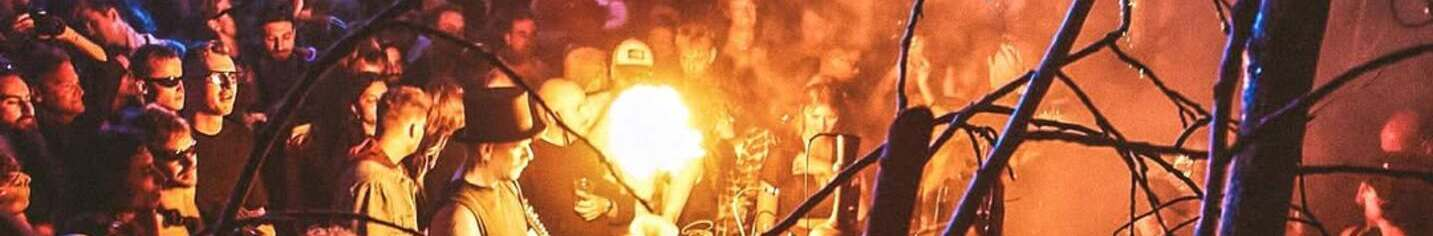
\includegraphics[width=\linewidth]{img/detail_crop.jpg}};
  \draw[brass, opacity=0.5, line width=0.4pt] (detailimg.north west) rectangle (detailimg.south east);
\end{tikzpicture}

\vfill
\noindent
{\color{hairline}\hrule height 0.4pt}
\vspace{1.5mm}
\noindent
{\labelfont\fontsize{8.6}{10}\selectfont%
  \cvlink{https://tromleorkestret.com}{tromleorkestret.com} \quad
  \cvlink{https://instagram.com/tromleorkestret}{instagram.com/tromleorkestret} \quad
  \cvlink{https://facebook.com/tromleorkestret}{facebook.com/tromleorkestret}}%
\hfill
{\labelfont\fontsize{7.6}{10}\selectfont\color{hairline} 01 / 02}

\clearpage

% ================================================================
%  PAGE 2
% ================================================================
\bgfill

\noindent
\begin{tabularx}{\linewidth}{@{}X r@{}}
{\fontsize{19}{19}\selectfont\itshape\bfseries\color{brightcream} Shows, People \& Rider} &
{\labelfont\fontsize{7.6}{10}\selectfont\color{muted}\MakeUppercase{Tromleorkestret --- Booking Sheet}}
\end{tabularx}

\vspace{2mm}
{\color{brass}\hrule height 0.6pt}
\vspace{6mm}

\noindent
\begin{minipage}[t]{0.54\linewidth}

  % ---- selected shows ----            %%% EDIT ME — add/remove rows freely
  \eyebrow{Selected Shows}\\[1mm]
  {\color{hairline}\hrule height 0.4pt}
  \vspace{1mm}
  {\serifreader\fontsize{9}{15}\selectfont\color{bodytext}
  \begin{tabularx}{\linewidth}{@{}X r@{}}
    Fusion Festival, Germany & {\labelfont\fontsize{8}{10}\selectfont\color{muted}Jun 2025}\\
    \arrayrulecolor{hairline!60}\hline
    Karrusel Festival, Denmark & {\labelfont\fontsize{8}{10}\selectfont\color{muted}Aug 2025}\\
    \hline
    Frigjort Festival, Denmark & {\labelfont\fontsize{8}{10}\selectfont\color{muted}Aug 2025}\\
    \hline
    Kultursalonerne Gisselfeld, Denmark & {\labelfont\fontsize{8}{10}\selectfont\color{muted}Aug 2024}\\
    \hline
    Bascherdeis Festival, Italy & {\labelfont\fontsize{8}{10}\selectfont\color{muted}Aug 2024}\\
    \hline
    Pumpehuset, Denmark & {\labelfont\fontsize{8}{10}\selectfont\color{muted}Sep 2023}\\
    \hline
    Bades\o en Festival, Denmark & {\labelfont\fontsize{8}{10}\selectfont\color{muted}Aug 2023}\\
    \hline
    Stjerner over Far\o, Denmark & {\labelfont\fontsize{8}{10}\selectfont\color{muted}Jul 2023}\\
    \hline
    Amager B\o rnemusikfestival, Denmark & {\labelfont\fontsize{8}{10}\selectfont\color{muted}Feb 2023}\\
    \hline
    ART by NIGHT, Denmark & {\labelfont\fontsize{8}{10}\selectfont\color{muted}Aug 2022}\\
    \hline
    Kulturnatten x Reffen, Denmark & {\labelfont\fontsize{8}{10}\selectfont\color{muted}Oct 2019}\\
    \hline
    Analogik + Tromleorkestret at Loppen, Denmark & {\labelfont\fontsize{8}{10}\selectfont\color{muted}Sep 2019}\\
  \end{tabularx}}

  \vspace{4mm}

  % ---- the ensemble ----              %%% EDIT ME — bios
  \eyebrow{The Ensemble}\\[1mm]
  {\color{hairline}\hrule height 0.4pt}
  \vspace{2mm}

  {\fontsize{10.6}{13}\selectfont\itshape\bfseries\color{brightcream} Hjalte Bested Hjorth}\\
  {\labelfont\fontsize{7.4}{9}\selectfont\color{brass}\MakeUppercase{Instrument Design, Composer \& Performer}}\\[1mm]
  {\serifreader\fontsize{8.9}{13}\selectfont\color{bodytext}
   A musician and composer with a background in robotics engineering,
   Hjalte is in charge of all the technical innovations and music
   composition for the project.\par}

  \vspace{3mm}

  {\fontsize{10.6}{13}\selectfont\itshape\bfseries\color{brightcream} Sofie Hjorth Schausen}\\
  {\labelfont\fontsize{7.4}{9}\selectfont\color{brass}\MakeUppercase{Special Effects, Visual Design \& Performer}}\\[1mm]
  {\serifreader\fontsize{8.9}{13}\selectfont\color{bodytext}
   Sofie has created the costumes and visual design of the project. In
   performance, she is mainly in control of live audio effects.\par}

\end{minipage}%
\hfill
\begin{minipage}[t]{0.42\linewidth}

  % ---- technical & hospitality rider ----   %%% EDIT ME — rider terms
  \eyebrow{Technical \& Hospitality Rider}\\[1mm]
  {\color{hairline}\hrule height 0.4pt}
  \vspace{1.5mm}

  % Each rider line is two [t]-aligned minipages side by side (label,
  % value), NOT a tabularx row --- tabularx/array centre multi-line p{}
  % cells against short ones by the row's mid-height, not by their top,
  % which is what threw the label/value rows out of line here. Add a new
  % line with \riderrow{Label}{Value text} on its own line below.
  \newcommand{\riderrow}[2]{%
    \noindent
    \begin{minipage}[t]{18mm}\rlabel{#1}\end{minipage}%
    \begin{minipage}[t]{\dimexpr\linewidth-18mm\relax}
      {\serifreader\fontsize{8.4}{12.5}\selectfont\color{bodytext}#2\par}
    \end{minipage}\\[2.2mm]%
  }

  \riderrow{Power}{Fully self-contained --- no venue power needed for a standard show. Multi-day festivals: trailer parking + 220V to recharge batteries.}
  \riderrow{Sound}{Own onboard PA; stereo DI line-out available if the venue system is preferred.}
  \riderrow{Footprint}{L130 $\times$ W120cm (W100cm with keyboard unmounted, remounted inside the venue) $\times$ H190cm. Weight $\approx$200kg.}
  \riderrow{Access}{Drivable path or crane to position. Rolls up/down gentle slopes; cannot be carried on stairs.}
  \riderrow{Catering}{Full catering incl. vegetarian option, and beverages with and without alcohol.}
  \riderrow{Lodging}{Free accommodation for overnight bookings.}
  \riderrow{Fee}{Scope-dependent --- ask for a quote.}

  \vspace{2mm}

  % ---- two photos side by side ----
  % pre-cropped to their box ratios in img/ --- see img/README.md before
  % swapping in a different source photo
  \noindent
  \begin{tikzpicture}
    \node[anchor=north west, inner sep=0pt] (ph1) at (0,0)
      {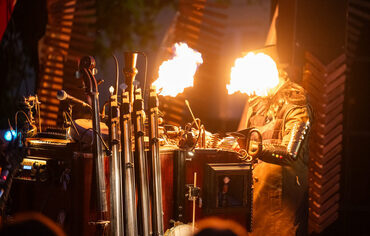
\includegraphics[width=47mm,height=30mm]{img/riderwide_crop.jpg}};
    \draw[brass, opacity=0.5, line width=0.3pt] (ph1.north west) rectangle (ph1.south east);

    \node[anchor=north west, inner sep=0pt, xshift=2mm] (ph2) at (ph1.north east)
      {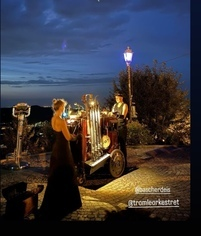
\includegraphics[width=25.5mm,height=30mm]{img/ridernarrow_crop.jpg}};
    \draw[brass, opacity=0.5, line width=0.3pt] (ph2.north west) rectangle (ph2.south east);
  \end{tikzpicture}

\end{minipage}

\vspace{5mm}

% ---- second photo strip ----
% pre-cropped to their box ratios in img/ --- see img/README.md before
% swapping in a different source photo
\noindent
\begin{tikzpicture}
  \node[anchor=north west, inner sep=0pt] (q1) at (0,0)
    {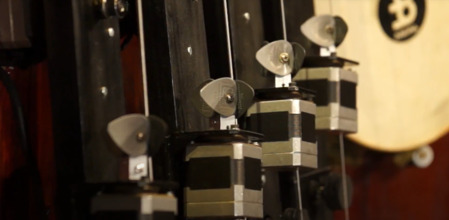
\includegraphics[width=57mm,height=28mm]{img/strip1_crop.jpg}};
  \draw[brass, opacity=0.5, line width=0.3pt] (q1.north west) rectangle (q1.south east);

  \node[anchor=north west, inner sep=0pt, xshift=2mm] (q2) at (q1.north east)
    {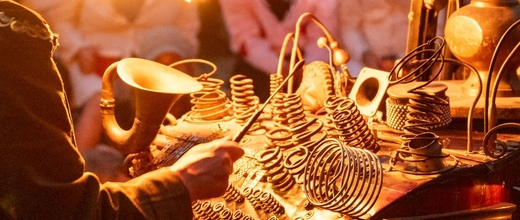
\includegraphics[width=66mm,height=28mm]{img/strip2_crop.jpg}};
  \draw[brass, opacity=0.5, line width=0.3pt] (q2.north west) rectangle (q2.south east);

  \node[anchor=north west, inner sep=0pt, xshift=2mm] (q3) at (q2.north east)
    {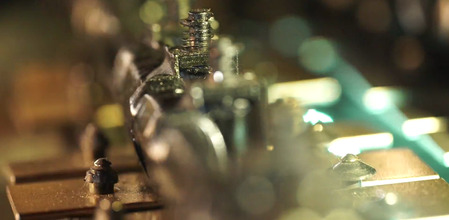
\includegraphics[width=57mm,height=28mm]{img/strip3_crop.jpg}};
  \draw[brass, opacity=0.5, line width=0.3pt] (q3.north west) rectangle (q3.south east);
\end{tikzpicture}

\vspace{3mm}

% ---- third photo strip ----
% pre-cropped to their box ratios in img/ --- see img/README.md before
% swapping in a different source photo
\noindent
\begin{tikzpicture}
  \node[anchor=north west, inner sep=0pt] (r1) at (0,0)
    {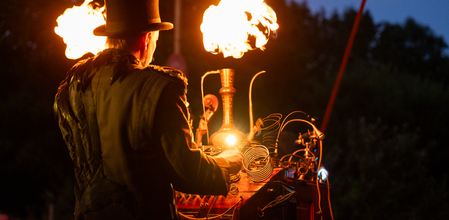
\includegraphics[width=57mm,height=28mm]{img/strip4_crop.jpg}};
  \draw[brass, opacity=0.5, line width=0.3pt] (r1.north west) rectangle (r1.south east);

  \node[anchor=north west, inner sep=0pt, xshift=2mm] (r2) at (r1.north east)
    {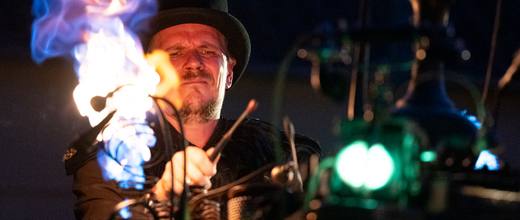
\includegraphics[width=66mm,height=28mm]{img/strip5_crop.jpg}};
  \draw[brass, opacity=0.5, line width=0.3pt] (r2.north west) rectangle (r2.south east);

  \node[anchor=north west, inner sep=0pt, xshift=2mm] (r3) at (r2.north east)
    {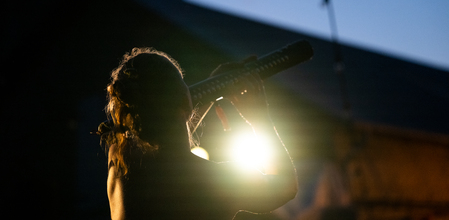
\includegraphics[width=57mm,height=28mm]{img/strip6_crop.jpg}};
  \draw[brass, opacity=0.5, line width=0.3pt] (r3.north west) rectangle (r3.south east);
\end{tikzpicture}

\vspace{5mm}

% ---- contact block ----              %%% EDIT ME — contact details
\noindent
\begin{tcolorbox}[
    enhanced, colback=brass!8!bg, colframe=brass!55, boxrule=0.5pt,
    arc=0pt, left=5mm, right=5mm, top=3.5mm, bottom=3.5mm
  ]
  \begin{tabularx}{\linewidth}{@{}X r@{}}
    \begin{minipage}[c]{0.6\linewidth}
      {\fontsize{12.5}{14}\selectfont\itshape\bfseries\color{brightcream} Tromleorkestret}\\[0.8mm]
      {\labelfont\fontsize{7.6}{11}\selectfont\color{muted}
       Att. Hjalte Bested Hjorth \textperiodcentered\ Bj\o rnekloen 374 st.tv,
       1440 K\o benhavn K \textperiodcentered\ CVR 37165107}
    \end{minipage}
    &
    \begin{minipage}[c]{0.38\linewidth}
      \raggedleft
      {\labelfont\fontsize{8}{15}\selectfont\color{cream}
       \cvlink{mailto:tromleorkestret@gmail.com}{tromleorkestret@gmail.com}\\
       \cvlink{tel:+4523282926}{+45 23 28 29 26}\\
       \cvlink{https://tromleorkestret.com}{tromleorkestret.com}\\
       \cvlink{https://instagram.com/tromleorkestret}{Instagram} \textperiodcentered\
       \cvlink{https://facebook.com/tromleorkestret}{Facebook} \textperiodcentered\
       \cvlink{https://youtube.com/@tromleorkestret}{YouTube}}
    \end{minipage}
  \end{tabularx}
\end{tcolorbox}

\vfill
{\color{hairline}\hrule height 0.4pt}
\vspace{1.5mm}
\noindent
\begin{tabularx}{\linewidth}{@{}X r@{}}
  {\labelfont\fontsize{7.2}{9}\selectfont\color{hairline} Booking \& press enquiries: tromleorkestret@gmail.com} &
  {\labelfont\fontsize{7.2}{9}\selectfont\color{hairline} 02 / 02}
\end{tabularx}

\end{document}
